\newchapstyle
\chapter{Current phase relations of graphene Josephson junctions in microwave circuits}
\label{chap:gJJ-CPR}

\blfootnote{
	\color{title}
	This chapter is based on previously unpublished data of the devices presented in Chapter~\ref{chap:gJJ}.
	%
	Data and code to reproduce the calculations and figures presented here can be found on Zenodo~\cite{schmidtDataCodeCurrent2020}.
}

\begin{abstract}
	We perform extensive analysis of graphene Josephson junctions embedded in microwave circuits.
	%
	By comparing a diffusive junction at \SI{15}{\milli\kelvin} with a ballistic one at \SI{15}{\milli\kelvin} and \SI{1}{\kelvin}, we are able to reconstruct the current-phase relation.
\end{abstract}

%% Start the actual chapter on a new page.
\newpage

\section{Introduction}

Josephson junctions are widely used in high frequency applications, such as quantum information processing and sensing.
%
There, they are being exploited as nonlinear inductors.
%
However, their nonlinear character can significantly differ from junction to junction depending on the intrinsic properties of the current-phase relation.
%
For the use of JJs in superconducting quantum information circuits, the junction nonlinearity has a major effect on the circuit requirements and capabilities~\cite{kringhojAnharmonicitySuperconductingQubit2018}.
%
While the CPR of gJJs has been studied in the DC regime before~\cite{englishObservationNonsinusoidalCurrentphase2016,nandaCurrentPhaseRelationBallistic2017}, and gJJs have been successfully incorporated in RF circuits~\cite{schmidtBallisticGrapheneSuperconducting2018,krollMagneticFieldCompatible2018,wangCoherentControlHybrid2019}, the influence of the non-sinusoidal CPR has not been studied in this regime.

Here, we analyze the influence of the CPR on the microwave performance of RF-circuit embedded gJJ and compare the influence of scattering transport and temperature.
%
Our circuit design allows in-situ, and even simultaneous, even DC and RF measurements, providing us with various measurement types to compare.
%
The results show the usefulness of combining DC and RF in the same circuits for funamental research on Josephson junction physics.

\section{Circuit characterization}

Our circuit consists of a DC-bias microwave cavity formed by a coplanar waveguide (CPW) which is shunted by a large capacitor at the input, and shorted to ground on the far end by a gate-voltage ($V_g$) tunable graphene Josephson junction (gJJ), cf. Fig.\ref{fig:figure1}(a) and Refs.~\cite{schmidtBallisticGrapheneSuperconducting2018,schmidtCurrentDetectionUsing2020,bosmanBroadbandArchitectureGalvanically2015c}.
%
The superconducting base layer and shunt capacitor metal layers consist of DC-sputtered molybdenum-rhenium (MoRe) on a sapphire substrate, while the shunt capacitr dielectric layer is PECVD-SiN.
%
The circuit is connected via a bias-T, allowing both DC and RF characterization in the same setup, and mounted on the millikelvin plate on a dilution refrigerator.
%
The gate voltage lead is fed through a shunt capacitor of the same geometry as the capacitor at the input in order to suppress RF radiation leaking in through or out of the gate line.

We measured two separate devices with nominally identical microwave circuits and junction designs:
%
One of the devices exhibited signatures ballistic DC-transport, which we will refer to as the \textit{ballistic device}, which is the device presented in the main text of Ref.~\cite{schmidtBallisticGrapheneSuperconducting2018}.
%
The other one, in lack of such features, will be called \textit{diffusive device}, and corresponds to the reference sample of Ref.~\cite{schmidtBallisticGrapheneSuperconducting2018}.
%
Both gJJ were designed to be \SI{5}{\micro\meter} wide and separate the NbTiN leads by a length of \SI{500}{\nano\meter}.
%
Gate tunability is achieved by placing a third NbTiN lead extending over the entire gJJ, separated by a bilayer of HSQ.

We extract the DC circuit parameters by applying a bias current to the JJ, using the CPW as a long capacitive lead.
%
All DC lines were equipped with $\pi$-filters in the room temperature battery powered electronics, as well as copper powder and two-stage RC filters thermally anchored to the millikelvin stage of the dilution refrigerator.
%
When exceeding a critical current, the JJ switches from the zero-voltage to the resistive state.
%
We record this switching current $I_s$ for varying gate voltages, as depicted in the top row of Fig.~\ref{fig:figure1} for the two devices at two different temperatures.
%
The DC switching current of the diffusive device ranges from a few \SI{100}{\nano\ampere} to \SI{5.5}{\micro\ampere}, similar to the hot ballistic device.
%
At base temperature, the maximum $I_s$ of the ballistic device reaches \SI{7.5}{\micro\ampere} for $V_g>V_{\rm CNP}$, while for p-doping the enhancement in $I_s$ is significantly smaller.

For high frequency signals, i.e. a few \si{\giga\hertz}, the gJJ behaves as a nonlinear inductor, with Josephson inductance
%
\begin{align}
L_J = \frac{\Phi_0}{2\pi}\left(\diff{I_J}{\delta}\right)^{-1},
\label{eq:LJgeneral}
\end{align}
%
where $\Phi_0$ is the magnetic flux quantum and $I_J(\delta)$ the current phase relation (CPR) between the phase difference $\delta$ across the JJ between two superconducting banks and the corresponding supercurrent $I_J$ flowing through the junction.
Depending on the impedance of the gJJ at the circuit resonance frequency, $Z_J=i\omega_0 L_J$, the fundamental mode hosted by the gJJ-terminated CPW varies between a $\lambda/2$ wave for $Z_J\rightarrow0$ and $\lambda/4$ for $Z_J\rightarrow\infty$.
%
Since the supercurrent in our gJJs cannot be fully suppressed, the maximum $L_J\lessapprox\SI{1}{\nano\henry}$, thus $Z_J\lessapprox1 <  Z_0\approx\SI{50}{\ohm}$ with the CPW impedance $Z_0$.
%
Our devices thus remain in the $\lambda/2$-resonator regime.

The device response is measured by recording the reflection coefficient $S_{11}$ using a vector network analyzer, which excites the device through a series of attenuators and a directional coupler, and measuring the reflected signal, amplified by low noise cryogenic and room temperature HEMTs. 
%
We fit the response using an analytical model (cf. Supplementary Sec.~\ref{sec:extraction}).
%
The measurements show a gate-tunable resonance frequency $f_0$ between \SIrange{7.0}{8.2}{\giga\hertz}, comparable for both devices, cf. bottom row of Fig.~\ref{fig:figure1}.
%
Due to the inverse nature of junction current and inductance, the large changes in $I_s$ for $V_g>V_{\rm CNP}$ only lead to minor changes in $f_0$ when comparing the hot and cold ballistic device.
%
On the other hand, even small changes in the significantly smaller $I_s$ for $V_g<V_{\rm CNP}$ significantly reduce $f_0$ in this regime.

\begin{figure}
	\centering
	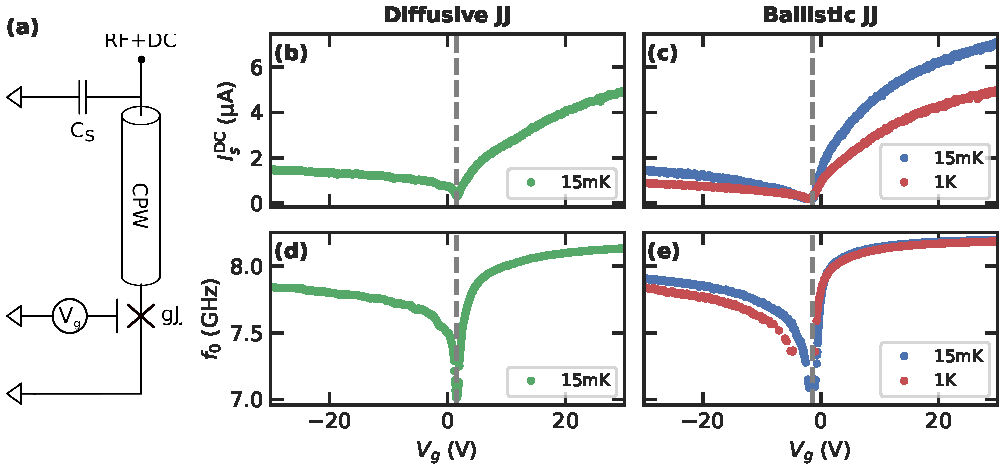
\includegraphics[width=\linewidth]{chapter-gJJ-CPR/figs/Figure1}
	\caption{
		\textbf{A graphene Josephson junction embedded in a DC bias microwave circuit.}
		%
		\textbf{(a)} Measurement schematic.
		%
		The gJJ shorts a coplanar waveguide transmission line to ground, which forms a gate-tunable $\lambda/2$-resonator.
		%
		\textbf{(b-e)} Switching currents (top row) for the diffusive \textbf{(b)} and ballistic Josephson junction \textbf{(d)}, at base-temperature of \SI{15}{\milli\kelvin} (blue) and at \SI{1}{\kelvin} (red).
		%
		Bottom row: Resonance frequencies versus gate voltage for the diffusive \textbf{(c)} and ballistic \textbf{(e)} device.
		%
		The gate-tunable Josephson inductance changes the boundary condition of the $\lambda/2$-resonator, thus changing the resonance frequency of the circuit.
		%
		Dashed grey lines indicate the charge neutrality point
	}
	\label{fig:figure1}
\end{figure}


\section{Measuring the Josephson inductance in DC and RF}

\begin{figure}
	\centering
	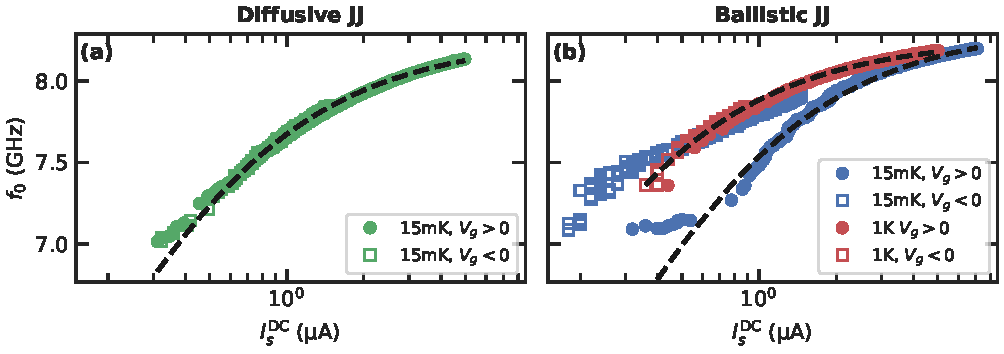
\includegraphics[width=0.583\linewidth]{chapter-gJJ-CPR/figs/Figure2}
	\caption{
		\textbf{Resonance frequency vs switching currents for two different gJJ devices.}
		%
		Both the diffusive device at low temperature \textbf{(a)} and the ballistic device at \SI{1}{\kelvin} (\textbf{(b)}, red) show monotonically increasing $f_0$ versus DC-extracted switching currents.
		%
		In contrast, for low temperatures, the ballistic gJJ (\textbf{(b)}, blue) exhibits multi-valued $f_0\left(I_s\right)$ for gate voltages larger (full circles) and smaller (empty squares) than the charge neutrality point.
		%
		The	multivalued behavior in the ballistic device at low temperature indicates a strong nonsinusoidal CPR and only allows for a fit for $V_g>0$, while this is not observed at higher temperature or for the diffusive device.
		%
		Dashed lines correspond to fits to Eq.~\ref{eq:Pogorzalek}.
	}
	\label{fig:figure2}
\end{figure}

The resonance frequency of a $\lambda/2$-resonator shorted to ground by a Josephson inductance can be approximated by
\begin{align}
f_0\left(I_b,I_c\right) = f_{\lambda/2} \frac{L_r+L_J\left(I_b, I_c\right)}{L_r +  2L_J\left(I_b, I_c\right)}
\label{eq:Pogorzalek}
\end{align}
%
with $L_r$ the bare CPW inductance and $f_{\lambda/2}$ the resonance frequency of the CPW without the JJ, see Supplementary Material Sec.~\ref{sec:validity}.
%
$I_b$ is the bias current flowing through CPW and the JJ, $I_c$ the critical current of the JJ.
%
We can immediately see that for small $L_J$, $f_0=f_{\lambda/2}$, while for $L_J\gg L_r$, $f_0=f_{\lambda/2}/2$.
%
Assuming a purely sinusoidal current-phase relation,
%
\begin{align}
I_J(\delta) = I_c\sin\delta,
\label{eq:CPR-sin}
\end{align}
%
the Josephson inductance can be extracted from the current phase relation via
%
\begin{align}
L_J = \frac{\Phi_0}{2\pi I_c \cos\delta}.
\label{eq:LJsin}
\end{align}
%
Depending on the exact shape of the CPR however, $L_J$, and with it $f_0$ can significantly deviate from the above equations, cf. Supplementary Fig.~\ref{fig:SMinfluence}.
%
Specifically, the CPR of gJJ are known to exhibit forward-skewing, where the skew is defined as the deviation of the CPR maximum from phase $\pi/2$, $S=2\delta_{\rm max}/\pi -1$.

As depicted in Fig.\ref{fig:figure2}, we fit the RF-measured $f_0$ versus the DC-measured $I_s^{\rm DC}$ using Eq.~\ref{eq:Pogorzalek} assuming a sinusoidal CPR, shown by the black dashed line.
%
Here, we assumed $\delta=0$ because the DC bias port was shorted to ground during measurement, and the RF excitation merely oscillates the phase around zero.
%
The fit converges for both the diffusive and the “hot” ballistic device.
%
On the other hand, at \SI{15}{\milli\kelvin}, the ballistic device exhibits multi-valued $f_0\left(I_s\right)$, as the resonance frequency and switching current follow different trends for p- and n-doping.
%
This is a first indication of a deviation of the CPR from Eq.\ref{eq:CPR-sin}.

%% How to formulate this in a good way?
%% DC-Is and assumption of sinusoidal CPR leads us to an estimated DC-Lj.
%% This value is smaller than the actually measured Lj
%% This can only be if the CPR is forward skewed because this enhances the true Lj while keeping Ic the same for the two cases.
%% To get the same Lj as for a sinusoidal CPR, DC-Is would need to be smaller.? But according to Figs1.2, 1.3 it would need to be larger???
%% TODO!

We can additionally directly compare the estimates for the junction critical current from our DC measurement, $I_s^{\rm DC}$, with the value calculated from our RF measurement of the resonance frequency via Eq.~\ref{eq:LJsin}, $I_c^{\rm RF}=I_c\left(L_J\left(f_0\right)\right)$. 
%
As shown in Fig.~\ref{fig:figure3}, our devices exhibit tunable supercurrent over almost two orders of magnitude range.
%
In the diffusive device, $I_s^{\rm DC}$ and $I_c^{\rm RF}$ match closely, but small deviations at the low and high end are visible, with $I_c^{\rm RF}$ resulting in values larger than expected from DC.
%
Similarly, the DC measurements of the ballistic device at \SI{1}{\kelvin} underestimate the critical current as extracted from RF for small values of $I_s^{\rm DC}$, but match remarkably well everywhere else.
%
At first glance, any forward skew in the CPR should lead to a drop in CPR slope.
%
Therefore, for the same value of $I_c$, $L_J$ should increase and $I_s^{\rm RF}<I_s^{\rm DC}$.
%
However, our fit results in the opposite behavior, cf. Supplementary Fig.~\ref{fig:SMinfluence}:
%
The fit model returns a larger $I_c$ than expected for a sinusoidal CPR, given that the data to be fitted has an underlying forward-skewed CPR.
%% I think I have this written down somewhere in one of the ipynb files?

At a temperature of \SI{15}{\milli\kelvin}, the ballistic device deviates significantly from the DC-calculations, especially at low currents and $V_g<0$.
%
Deviations at large $I_c$ are less obvious, presumably due to the fact that in this regime, $L_J \ll L_r$ and the Josephson inductance has only minor effect on $f_0$.

This shows that extrapolation of a value for $L_J$ at microwave frequencies from DC measurements can lead to severe discrepancies.
%
In order to examine the underlying mechanisms further, we continue by studying the power and bias current dependence of our circuit.

\begin{figure}
	\centering
	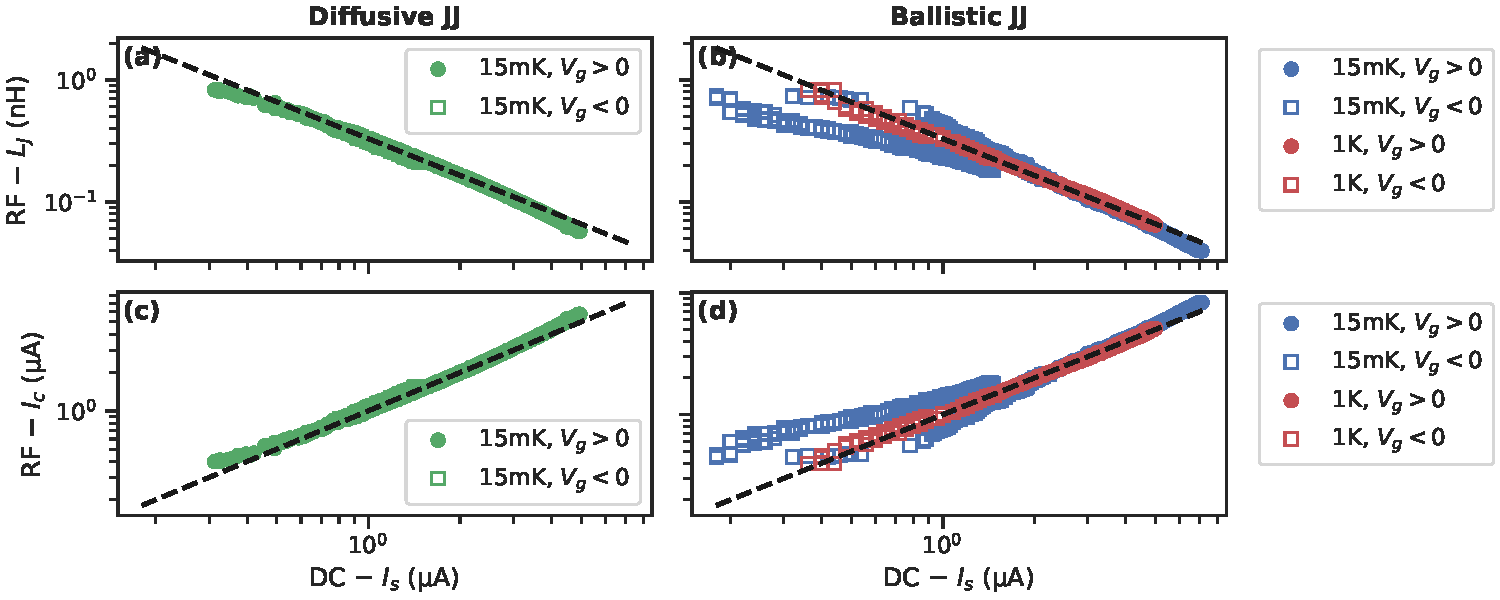
\includegraphics[width=0.583\linewidth]{chapter-gJJ-CPR/figs/Figure3}
	\caption{
		\textbf{Comparing switching and critical currents.}
		%
		RF-extracted critical current versus DC-measured switching current for the diffusive device at \SI{15}{\milli\kelvin} \textbf{(a)} and the ballistic device at \SI{15}{\milli\kelvin} and at \SI{1}{\kelvin} (\textbf{(b)}, blue and red, respectively).
		%
		Dashed line corresponds to DC-measured $I_s$.
		%
		Both scattering in the JJ as well as elevated temperatures reduce the deviation from RF and DC data.
	}
	\label{fig:figure3}
\end{figure}

\section{Reconstructing the current phase relation}

\subsection{Anharmonicity of a gJJ RF circuit}

The nonlinear inductance of a Josephson junction consequently introduces nonlinear behaviour of the overall circuit.
%
Depending on the exact circuit design, this nonlinearity is more or less diluted, yet finite so-called anharmonicity $\beta$, i.e. deviation from the ideal case of pure LC-resonator behavior, remains.
%
Our circuit architecture allows us to extract this quantity directly and to calculate the expected CPR skew:

We can observe the anharmonicity of our DC bias circuit terminated with the diffusive gJJ by performing $S_{11}$ measurements at high drive powers for a series of different gate voltages, as shown in Fig.~\ref{fig:figure4}.
%
At very low drive powers, the circuit response can be described by a purely harmonic oscillator.
%
As the drive power increases, the resonance frequency experiences a down-shift, and both amplitude and phase of $S_{11}$ start to get skewed towards lower frequencies.
%
Once the drive power exceeds a critical threshold, the resonator response bifurcates, which can be seen by the discontinuity in the data.
%
For comparison, all other measurements were performed at fixed drive power of \SI{-131.4}{dBm}, still in the linear regime.

We can model the data by solving the equation of motion of a harmonic oscillator with an additional third order term in the cavity field with  amplitude $\beta$, as detailed in Supplementary Material Sec.~\ref{sec:SMduffing}.
%
Additionally, best agreement between data and model is reached for nonlinear dissipation in the form of increasing internal linewidth with drive power, cf. Supplementary Fig.~\ref{fig:SMpower}.
%
This is in contrast with circuits incorporating standard aluminum oxide JJs, where nonlinear dissipation with increasing power is usually absent~\cite{boakninDispersiveMicrowaveBifurcation2007b}.

There are several dissipation mechanisms known in superconducting microwave circuits that depend on drive power include heating, dielectric losses, or subgap losses.
%
Heating of the circuit itself is unlikely due to the close match between data and model, and the fact that $f_0$ should tune significantly stronger, since $I_c$ should also be reduced by elevated temperatures, with potentially significant influence on $f_0$, c.f. Fig.~\ref{fig:figure1}, which we did not observe for any of the gate voltages.

Dielectric losses due to electric dipoles, such as two-level systems, are unlikely the source of observation, as these are known to be predominantly activated for decreasing excitation voltages~\cite{martinisDecoherenceJosephsonQubits2005c,oconnellMicrowaveDielectricLoss2008a,gunnarssonDielectricLossesMultilayer2013}.
%
Additionally, there is only dielectric volume present at the shunt capacitor dielectric and the gJJ (encapsulating BN and HSQ top-gate), where the circuit has voltage nodes and voltage fluctuations are therefore expected to have negligible effects.

We therefore attribute the source of the observed nonlinear damping to low-lying subgap states within the induced superconducting gap in the gJJ.
%
Loss mechanisms in similar SNS systems, with normal metal weak links, have shown similar effects~\cite{fuechsleEffectMicrowavesCurrentPhase2009,dassonnevilleDissipationSupercurrentFluctuations2013}, but they have not been observed before in gJJ.
%
We populate them as we increase the drive power, resulting in an increase in internal loss rate, cf. Supplementary Fig.~\ref{fig:SMFig-lossrates}.

We compare the measured value of $\beta$ with the one expected from a CPW shorted to ground by a Josephson junction, which is given by
\begin{align}
\beta=-\frac{f_0}{2} \left(\frac{L_J}{L_r+L_J}\right)^3\ ,
\label{eq:anharmonicity}
\end{align}
%
where we have followed the same notation as in the earlier equations~\cite{wilsonPhotonGenerationElectromagnetic2010b,zhouHighgainWeaklyNonlinear2014}.
%
As expected, assuming a sinusoidal CPR and using $I_s^{\rm DC}$ to calculate $L_J$ overestimates the anharmonicity, cf. Fig.~\ref{fig:figure4}(d), while Eq.~\ref{eq:anharmonicity} and the data match better for $I_c^{\rm RF}$.
%
In a non-sinusoidal CPR, the Josephson inductance is less nonlinear, which reduces the anharmonicity, resulting in a correction factor of
\begin{align}
\frac{\beta^\prime}{\beta} =  1-\frac{3}{4}\frac{\sum_i\tau_i^2}{\sum_i\tau_i} \rightarrow 1-\frac{3}{4}\tau 
\label{eq:anh_nonsin}
\end{align}
%
where the limes holds for an average $\tau$ of the ensemble of transmission channels~\cite{kringhojAnharmonicitySuperconductingQubit2018}.
%
We calculate the ratio $\beta_{\rm meas}/\beta_{I_s}\approx0.57$, resulting in an estimated average channel transmission of $\tau\approx0.24$ or a corresponding CPR forward skew $S\approx0.045$ for the diffusive gJJ device, which slightly deviates from a purely sinusoidal CPR, as expected.
%
Power spectra for the ballistic gJJ were not recorded.

\begin{figure}
	\centering
	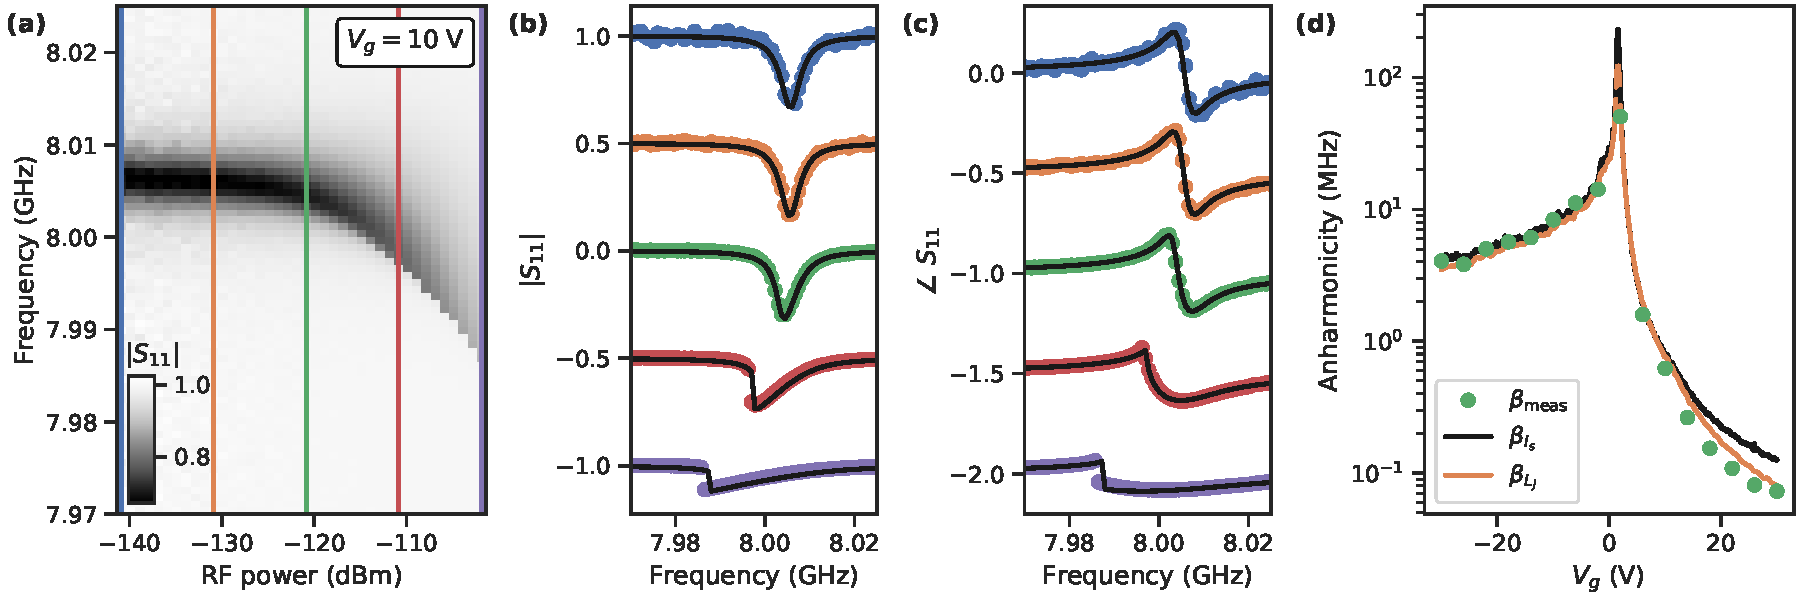
\includegraphics[width=\linewidth]{chapter-gJJ-CPR/figs/Figure4}
	\caption{
		\textbf{Power dependence of a nonlinear microwave device with diffusive gJJ.}
		%
		\textbf{(a)} Absolute value of the reflection coefficient $S_{11}$ versus frequency for increasing drive power.
		%
		Due to the Kerr nonlinearity, the resonator experiences a downshift and bifurcation at elevated drive powers.
		%
		Solid lines indicate linecuts in \textbf{(b)} and \textbf{(c)}.
		%
		\textbf{(b-c)} Absolute value \textbf{(b)} and phase \textbf{(c)} of $S_{11}$ for varying drive power as indicated in \textbf{(a)}.
		%
		Black lines are fits.
		%
		\textbf{(d)} Anharmonicity vs gate voltage.
		%
		Dots: data as extracted from fits as in \textbf{(b-c)}, orange line: model using $I_s^{\rm DC}$, green: model using $L_J$.
		%
		The overestimation of the anharmonicity of the $I_s^{\rm DC}$ for high gate voltages is consistent with and confirms a non-sinusoidal CPR.
	}
	\label{fig:figure4}
\end{figure}

\subsection{Current bias dependence}

A second way of reconstructing the CPR is by the means of analyzing the bias current dependence of the high frequency circuit response, as this allows for a direct measure of $L_J(\delta(I_b))))$.
%
Compared to the sinusoidal case, a more realistic model for the CPR of our devices than Eq.~\ref{eq:CPR-sin} is the one for a ballistic point contact as a function of transparency $\tau$ and temperature $T$:
%
\begin{align}
I_J(\delta,\tau,T) = \frac{\pi\Delta_0}{2 e R_n} \frac{\sin\delta}{\sqrt{1 - \tau \sin^2\delta / 2}} \tanh\left[\frac{\Delta_0}{k_B T} \sqrt{1 - \tau \sin^2\delta / 2}\right]\ ,
\label{eq:CPR-ball}
\end{align}
%
with the superconducting energy gap at zero temperature $\Delta_0$, the Boltzmann constant $k_B$ and normal state resistance $R_n= R_q/N = h/(Ne^2)\approx \SI{25.812}{\kilo\ohm} / N$~\cite{golubovCurrentphaseRelationJosephson2004a,leeUltimatelyShortBallistic2015}.
%
Here, $R_q$ denotes the quantum Hall resistance and $N$ the number of conducting channels.


The transparency $\tau$ is, similar to Eq.~\ref{eq:anh_nonsin}, taken as an average transmission probability of the $N$ channels.
%
With a normal state resistance of or devices ranging between \SIrange{35}{350}{\ohm} (depending on gate voltage), we estimate around 74 to 740 conducting channels.
%
This justifies the use of a single averaged transparency parameter $\tau$.
%
Equipped with this general CPR, we model the bias current dependence of both the ballistic and diffusive device at \SI{15}{\milli\kelvin} using Eqs.~\ref{eq:Pogorzalek} and \ref{eq:LJgeneral} with the assumption of Eq.~\ref{eq:CPR-ball}.
%
As the transparency increases, the CPR gets flatter, significantly increasing $L_J$ and thus the cavity tuning, cf. Fig.~\ref{fig:SMinfluence}
%
For details on the fitting algorithm, see the Supplemental Material Sec.~\ref{sec:fitbiascurrent}.


Our model accurately reproduces the data for all measured gate voltages, cf. Fig.~\ref{fig:figure5}(a), which allows us to extract a CPR-transparency parameter $\tau(V_g)$, as plotted in Fig.~\ref{fig:figure5}
(b).
%
We extract an average channel transmission $\tau_{\rm diff}=0.17\pm0.08$ and $\tau_{\rm ball}=0.88\pm0.03$.
%
This corresponds to a forward skew of $S_{\rm diff}=0.03_{-0.02}^{+0.01}$ and $S_{\rm ball}=0.34_{-0.05}^{+0.03}$ for the diffusive and ballistic device, respectively.
%
These values agree with the ones extracted from the power dependence within their error bars, confirming the skew CPR.
%
We note that they are also comparable to the results obtained from DC-measurements of the CPR~\cite{englishObservationNonsinusoidalCurrentphase2016,nandaCurrentPhaseRelationBallistic2017}.

\begin{figure}
	\centering
	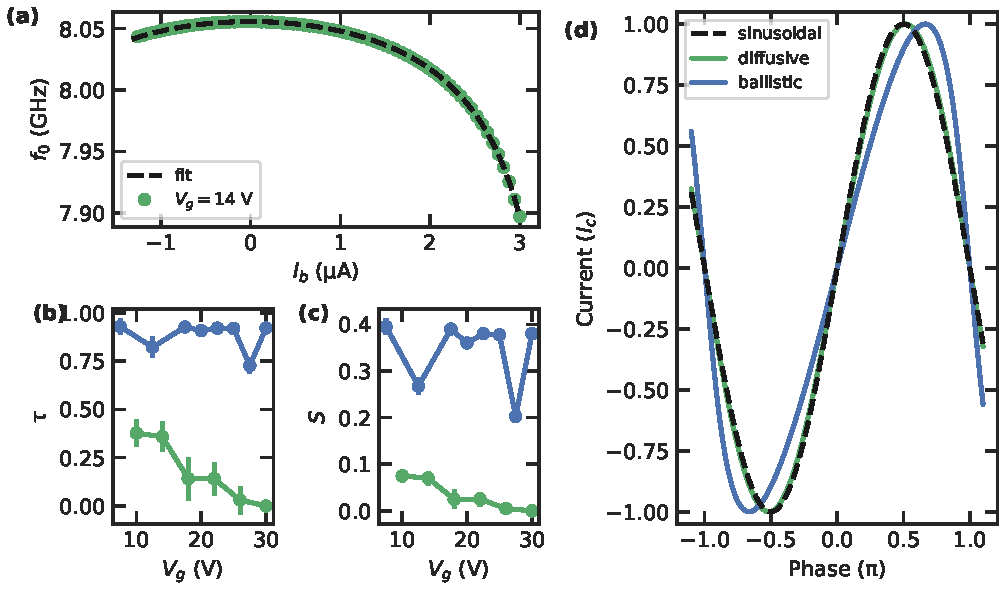
\includegraphics[width=\linewidth]{chapter-gJJ-CPR/figs/Figure5}
	\caption{
		\textbf{Extracting the current phase relation from current-biasing the gJJ microwave circuit.}
		%
		Fitting the bias current dependence \textbf{(a)}, we can extract the junction transparency \textbf{(b)} and corresponding CPR skew \textbf{(c)} for the diffusive (green) and ballistic (blue) gJJ device versus gate voltage.
		%
		\textbf{(d)} Reconstructed current-phase relation for the diffusive (green) and ballistic (blue) device.
		%
		The large transparency of the ballistic JJ leads to significant forward skewing, while the relatively low transparency of the diffusive JJ only results in minor skewing.
	}
	\label{fig:figure5}
\end{figure}

\section{Conclusion}

We plot the thus reconstructed current phase relations of both the ballistic and diffusive gJJ in Fig.~\ref{fig:figure5}(d).
%
While the relatively small forward skew of the diffusive device only deviates slightly from the case of a perfectly sinusoidal CPR, the ballistic device shows significant forward skewing.
%
We would like to point out that even though the skew in the diffusive case is only minor, our RF circuit is highly sensitive to these small changes, making its use competitive with DC-measurements of the CPR by using asymmetric SQUIDs or pickup loops.

Our circuit architecture thus is an attractive candidate for analyzing the CPR of exotic JJs, such as ferromagnetic or topological ones~\cite{golubovCurrentphaseRelationJosephson2004a,sochnikovNonsinusoidalCurrentPhaseRelationship2015,stoutimoreSecondHarmonicCurrentPhaseRelation2018,assoulineSpinOrbitInducedPhaseshift2019}.
%
Moreover, the influence of high microwave powers on the CPR can be studied straightforward, as this only requires repeating the bias current measurements at various powers.
%
Additionally, the combination of bias current and power dependence should allow to trace out a larger part of the CPR than just around zero phase.
%
Finally, on top of a built-in method of reconstructing phase-sensitive information, incorporating asymmetric gate-tunable SQUIDs instead of single JJs would enable a further in-situ method of probing and reconstructing the CPR.

For the case of graphene Josephson junctions in cQED applications, they seem rather unfeasible for relatively high-power devices such as quantum-limited parametric amplification, as the inherent nonlinear damping due to the subgap states limits the maximum drive power.
%
Future research on improvements towards a hard superconducting gap could advance these applications.
%
Nevertheless, using gJJs in low-power circuits, such as transmon qubits, is still an attractive alternative to the established aluminum oxide JJs, as the gate-tunability and potential sweet spots in the Fabry-Pérot regime could allow for long qubit coherence times.

%%%%%%%%%%%%%%%%%%%%%%%%%%%%%%%%%%%
% Insert SM.tex contents here

\pagebreak
\clearpage
%\widetext

%\setcounter{equation}{0}
%\setcounter{figure}{0}
%\setcounter{table}{0}
%\setcounter{page}{1}
%\setcounter{section}{0}

%\renewcommand{\thepage}{S\arabic{page}}
%\renewcommand{\thesection}{S\Roman{section}}
%\renewcommand{\thetable}{S\Roman{table}}
%\renewcommand{\thefigure}{S\arabic{figure}}
%\renewcommand{\theequation}{S\arabic{equation}}
%\renewcommand{\bibnumfmt}[1]{[S#1]}
%\renewcommand{\citenumfont}[1]{S#1}

\section{Supplementary Material: Current phase relations of graphene Josephson junctions in microwave circuits}

\subsection{Internal loss rate dependence on bias current, drive power and gate voltage}\label{sec:kintib}

The internal loss rate of our circuit depends on various parameters.

\begin{itemize}
	\item \textbf{Bias current dependence, cf. Fig~\ref{fig:SMFig-lossrates}(a)}
	\item \textbf{Drive power dependence, cf. Fig~\ref{fig:SMFig-lossrates}(b)}
	\item \textbf{Gate voltage dependence, cf. Fig~\ref{fig:SMFig-lossrates}(c)}
\end{itemize}

\begin{figure}
	\centering
	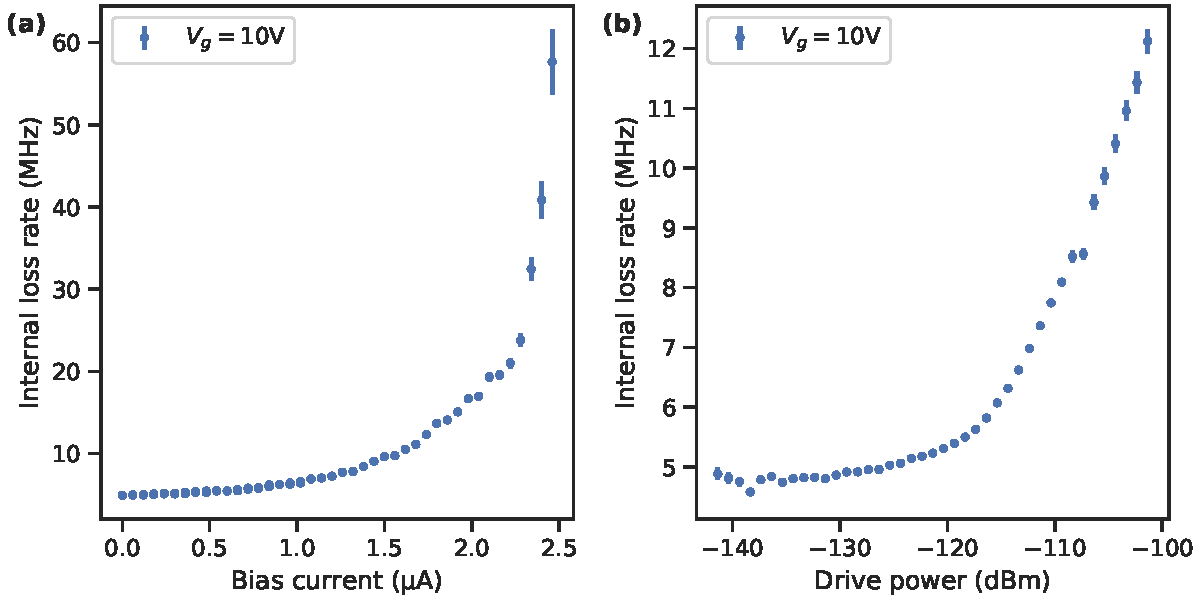
\includegraphics[width=\linewidth]{chapter-gJJ-CPR/figs/SMFigure-lossrates}
	\caption{
		\textbf{Internal loss rate for varying gate voltage (a), increasing bias current (b) and drive power (c).}
		%
		Higher losses around the CNP and for $V_g<0$ are presumably due to a higher number of subgap states.
		%
		Increasing loss rate with bias current could originate from either low-frequency noise or phase slip events.
		%
		An increase in $\kappa_i$ with drive power could be due to subgap states in the gJJ.
	}
	\label{fig:SMFig-lossrates}
\end{figure}


\subsection{Estimation of the fridge attenuation}\label{sec:attenuation}
The HEMT noise power is given by
%
\begin{align}
P_{\rm HEMT}=10\log\left(\frac{k_B T_{\rm HEMT}}{\si{\milli\watt}}\right) + 10\log\left(\frac{\Delta f}{\si{\hertz}}\right)\ ,
\label{eq:HEMT}
\end{align}
%
with the Boltzmann constant $k_B$, the noise temperature of the HEMT $T_{\rm HEMT}=\SI{2}{\kelvin}$ as specified by the manufacturer and the measurement bandwidth $\Delta f=\SI{100}{\hertz}$ resulting in $P_{\rm HEMT}\approx\SI{-175.59}{dBm}$.

By averaging over a few $S_{11}$ traces taken with the VNA in an area unaffected by our DUT, i.e. off-resonant to the cavity and thus leaving the background unaltered in power, we extract an average signal and standard deviation which we use to define the signal-to-noise ratio at the VNA, $\text{SNR}_\text{VNA}=\SI{34.5}{\decibel}$ for a VNA output power of \SI{0}{dBm}.

attenuation of \SI{129.3}{dB} of our VNA input line, assuming $X=\SI{2}{dB}$ of cable loss between sample and HEMT

\subsection{Extraction of $I_s^{\rm DC}$ and $f_0$}\label{sec:extraction}

The DC switching current (Fig.~\ref{fig:figure1}(b,c)) is taken as the current at which $\partial V/\partial I_b$ is maximum, where $V$ is the measured voltage.
%
Noise or interference on the DC lines could lead to a reduction of the measured $I_s$ compared to the true $I_c$.
%
To get a more accurate estimation of $I_c$ together with a good understanding of the noise sources, switching histograms are the preferred measurement method.
%
The necessary setup was however not available at the time of measurement.

To extract resonance frequency and loss rates from the RF data, we fit the reflection coefficient to the following model (cf. Ref.~\cite{bosmanBroadbandArchitectureGalvanically2015c} for a derivation):
%
\begin{align}
S_{11}(\omega) = -1+\frac{2\kappa_e}{\kappa+2i\Delta},
\end{align}
%
where $\kappa=\kappa_e+\kappa_i$ denoting the total, external and internal loss rates, respectively, and $\Delta=\omega-\omega_0$ with resonance frequency $\omega_0=2\pi f_0$.
%
The measured $S_{11}$ is usually distorted by a setup-related microwave background of the following shape:
\begin{align}
B(\omega) = \left(a+b\omega+c\omega^2\right)e^{i\left(a^\prime+b^\prime\omega\right)},
\end{align}
%
and with additional rotation by angle $\theta$ in the complex plane, the measured $S_{11}^\prime$ is:
\begin{align}
S_{11}^\prime(\omega)=B(\omega)\left(e^{i\theta}\left(S_{11}(\omega)+1\right)-1\right)
\end{align}
%
The origin of the microwave background and phase rotations are impedance mismatches in the wiring originating from various non-ideal circuit elements (e.g. connectors, attenuators, directional couplers).
%
Standing waves can form in some segments of the wiring which interfere with the measured signal.

For the gate voltage sweeps (Fig.~\ref{fig:figure1}(d,e)), we pick the measurement trace at the CNP as the one with only background signal, as the RF resonance is extremely broad and effectively not present anymore.
%
We then divide the other traces by this background, resulting in a much cleaner signal.

For measurements based on bias current sweeps, cf. Fig~\ref{fig:figure5}(a), we take the RF background at $I_b>I_s$ at which the JJ switched to the normal state and the RF resonance is removed from the measurement and divide it off the cases at which there is a circuit resonance.

In order to remove RF background from the power dependence, we mask the regions in which there are resonances for the various powers and gate voltage setpoints, and average the remaining traces.
%
This way, we obtain a power and frequency map of the RF background, which we use for removing background signal from power traces, such as the one in Fig.~\ref{fig:figure4}(a).

\subsection{Derivation and validity of Eq.~\ref{eq:Pogorzalek}}\label{sec:validity}

\begin{figure}
	\centering
	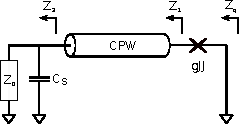
\includegraphics[width=0.5\linewidth]{chapter-gJJ-CPR/figs/rfderivation}
	\caption{
		\textbf{Derivation of resonance frequency.}
		%
		We define the three impedances $Z_1$, $Z_2$ and $Z_q$ as seen from the CPW towards the input port, from the gJJ towards the CPW, and as the parallel circuit impedance.
	}
	\label{fig:rfderivation}
\end{figure}

We can derive an expression for the circuit resonance frequency depending on the other parameters by using the impedances defined in Fig.~\ref{fig:rfderivation}.
%
The circuit impedance as seen from the JJ towards the CPW, $Z_1$, the input impedance as seen from the CPW towards the input port, $Z_2$, and the overall parallel circuit impedance $Z_q$ are defined as follows:
%
\begin{align}
Z_1 &= Z_0 \frac{Z_2+Z_0\tanh\gamma l}{Z_0+Z_2\tanh\gamma l} \\
Z_2 &= \left(\frac{1}{Z_{C_s}}+\frac{1}{Z_0}\right)^{-1} = \left(i\omega C_s+\frac{1}{Z_0}\right)^{-1} \\
Z_q &= \left(\frac{1}{Z_{JJ}}+\frac{1}{Z_1}\right)^{-1} = \left(\frac{1}{i\omega L_J}+\frac{1}{Z_1}\right)^{-1}\ ,
\end{align}
%
with the CPW length $l$, the complex CPW loss per unit length $\gamma=\alpha+i\beta$, and the transmission line impedance $Z_0$.
%
Assuming negligible losses in the CPW, $\gamma l\approx i\beta l = i\pi\omega_0/\omega_r$ (i.e. the CPW only acts as a phase shifter) on resonance.
%
Using $\tanh(iz)=i\tan(z)$, the resonance condition of the above circuit is for the imaginary part of the admittance $Y=1/Z_q=0$, which yields
%
\begin{align}
0 = \Im \left[ \frac{1}{i\omega_0 L_J} + \frac{1}{Z_0}\frac{Z_0+iZ_2\tan\left(\pi\omega_0/\omega_r\right)}{Z_2+iZ_0\tan\left(\pi\omega_0/\omega_r\right)}\right]
\label{eq:SolAnalytical}
\end{align}
%
The solution of this equation for $\omega_0$ is plotted as solid line in Fig.~\ref{fig:SMval}(a).
%
We can approximate the above by a similar method as the authors of Refs.~\cite{wallquistSelectiveCouplingSuperconducting2006a,wustmannParametricResonanceTunable2013,pogorzalekHystereticFluxResponse2017}:
%
Assuming $Z_2\approx 0$ and expanding the tangent, we arrive at the expression stated in Eq.~\ref{eq:Pogorzalek} which is plotted as dashed line in Fig.~\ref{fig:SMval}(a).
%
We find that for all values of $L_J$, including the range in our experiments, the approximation differs by no more than \SI{1}{\percent} from the analytical solution, regardless of JJ to CPW impedance, cf. Figs.~\ref{fig:SMval}(b-c).


\begin{figure}
	\centering
	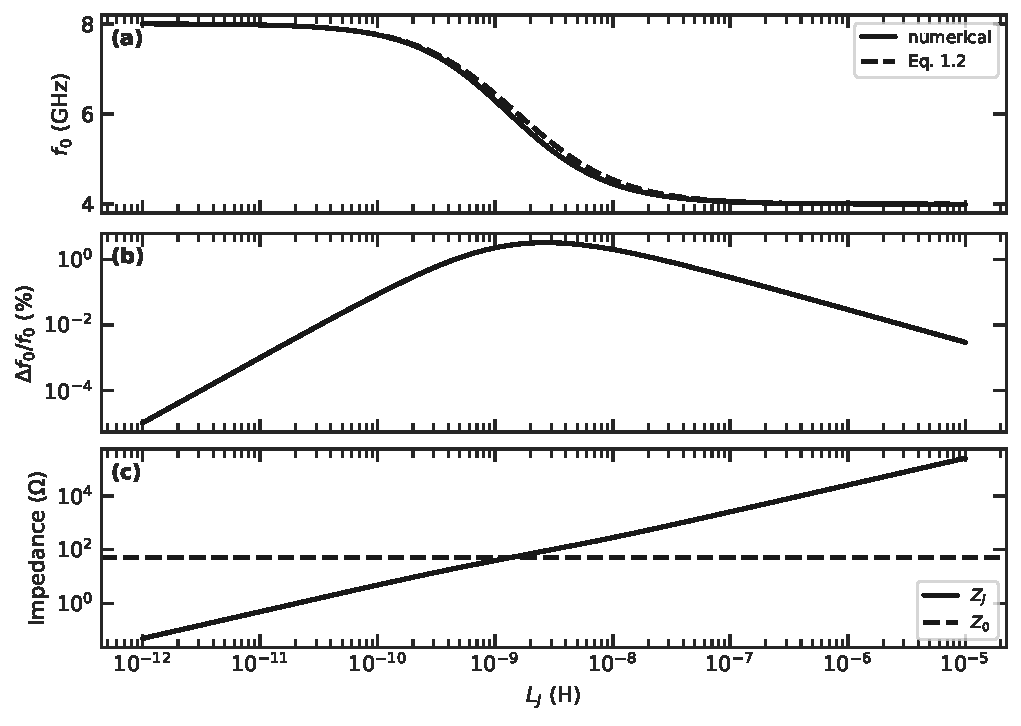
\includegraphics[width=0.5\linewidth]{chapter-gJJ-CPR/figs/SMFigure-validity}
	\caption{
		\textbf{Validity of Eq.~\ref{eq:Pogorzalek}.}
		%
		The equation used for modeling $f_0$ of the microwave circuit is an approximation to the true value.
		%
		\textbf{(a)} Resonance frequency as calculated using the  (solid) and using Eq.~\ref{eq:Pogorzalek} (dashed) for increasing Josephson inductance.
		\textbf{(b)} Relative difference between the two resonance frequencies.
		%
		\textbf{(c)} Impedance of the JJ (solid) and CPW impedance (dashed).
		%
		The approximation is in acceptable agreement with the full model regardless of $Z_J/Z_0$.
	}
	\label{fig:SMval}
\end{figure}


\subsection{Circuit parameters}

The values of the bare CPW resonator frequency and inductor are listed in Tab.~\ref{tab:frLr}.

\begin{table}[!h]
	\centering
	\caption{\textbf{Circuit parameters as extracted for the various measurements}}
	\begin{tabular}{|c|c|c|c|c|c|}
		\hline\hline
		& \multicolumn{2}{c|}{Diffusive JJ} & \multicolumn{3}{c|}{Ballistic JJ}  \\
		Temperature & \multicolumn{2}{c|}{\SI{15}{\milli\kelvin}} & \multicolumn{2}{c|}{\SI{15}{\milli\kelvin}} & \SI{1}{\kelvin} \\
		Measurement type & $V_g$ sweep & $I_b$ sweep & $V_g$ sweep & $I_b$ sweep & $V_g$ sweep \\
		\hline
		$f_{\lambda/2}$ (\si{\giga\hertz}) & $8.256878$ & $8.252736$ & $8.339123$ & $8.286517$  & $8.280240$ \\
		$L_r$ (\si{\nano\henry}) & $4.000$ & $3.857$ & $2.757$ & $3.622$ & $5.608$ \\
		\hline\hline
	\end{tabular}
	\label{tab:frLr}
\end{table}

\subsection{Fitting procedure for extracting $\beta$ from power dependence}\label{sec:SMduffing}

Following the method described in Ref.~\cite{schmidtCurrentDetectionUsing2020}, the equation of motion of the amplitude field $\alpha(t)$ of a resonator with weak anharmonicity $\beta$ written in the frame rotating with the drive $S_{\rm in}$ is given by
%
\begin{align}
\dot{\alpha} = \left[ -i \left( \Delta+\beta\abs{\alpha}^2 \right)-\frac{\kappa}{2} \right]\alpha + \sqrt{\kappa_\text{e}} S_\text{in}\ ,
\label{eq:Duffing-EOM}
\end{align}
%
from which the steady-state solution $\dot{\alpha_0}=0$ results in the following polynomial function,
% 
\begin{align}
\beta^2 \alpha_0^6 + 2\Delta\beta\alpha_0^4 + \left(\Delta^2+\frac{\kappa^2}{4}\right)\alpha_0^2 - \kappa_\text{e} \abs{S_{\rm in}}^2 = 0\ ,
\label{eq:polynom}
\end{align}
%
which we can solve numerically and use to calculate the expected reflection coefficient,
\begin{align}
S_{11}=-1-\frac{\sqrt{\kappa_e}}{S_{\rm in}}\alpha_0\ .
\label{eq:S11anh}
\end{align}
%
We reduce the number of free parameters from five to two by fixing $\omega_0$ and $\kappa_e$ as the values extracted at lowest drive power and calculating $S_{\rm in}$ from the fridge attenuation, see Supplementary Section Sec.~\ref{sec:attenuation}.
%
The remaining parameters are $\beta$ and $\kappa_i$, where the internal loss rate can in fact depend on the drive power, $\kappa_i=\kappa_i(S_{\rm in})$.
%
Fixing the loss rate to be constant throughout the fit does not lead to a good fit to the data, as shown in Fig.~\ref{fig:SMpower}.
%
Our algorithm first fits the measured data to return constant $\beta$ and $\kappa_i$, and uses these as initial values for a fit to extract the power dependent loss rate, shown in Fig.~\ref{fig:SMFig-lossrates}.

\begin{figure}
	\centering
	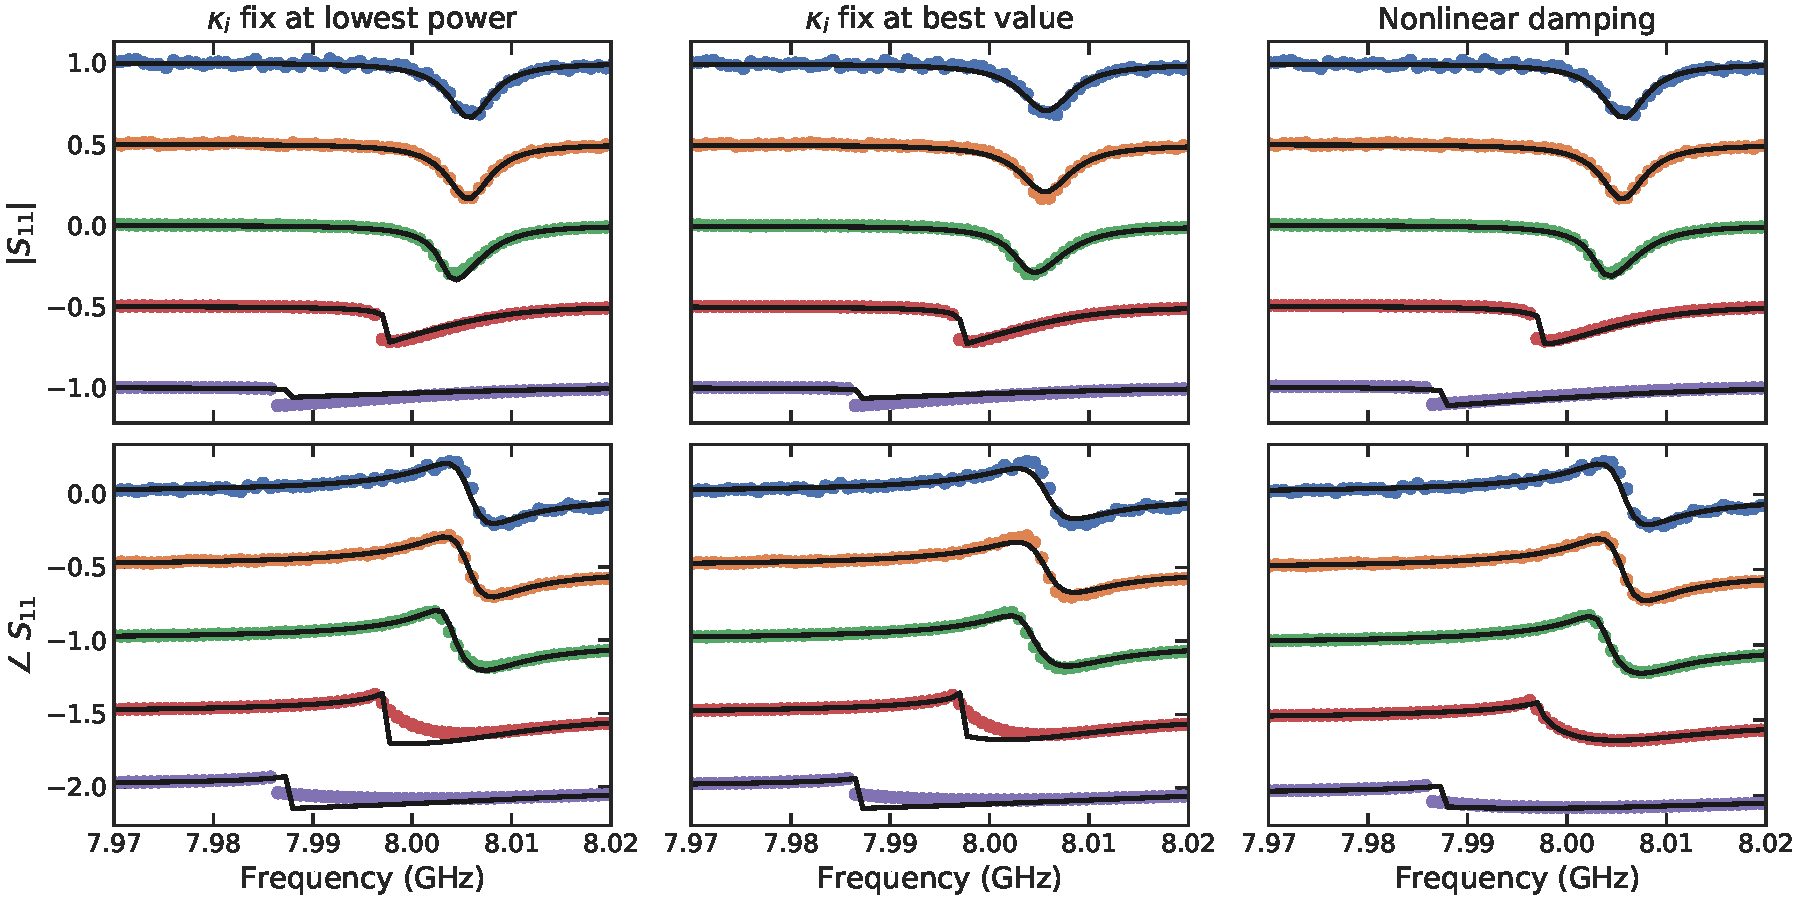
\includegraphics[width=\linewidth]{chapter-gJJ-CPR/figs/SMFigure-power}
	\caption{
		\textbf{Anharmonicity fit assuming different cases for $\kappa_i$.}
		%
		Fixing $\kappa_i$ to be the value at lowest drive power (first column) results in significantly worse fit than introducing it as constant, but free parameter (second column).
		%
		However, best agreement between data and model is reached when introducing nonlinear damping (third column and Fig.~\ref{fig:figure4}).
		%
		Linecuts and colors correspond to the ones in Fig.~\ref{fig:figure4}.
	}
	\label{fig:SMpower}
\end{figure}

\subsection{Fitting procedure for extracting $\tau$ from bias-current dependence}\label{sec:fitbiascurrent}

\begin{figure}
	\centering
	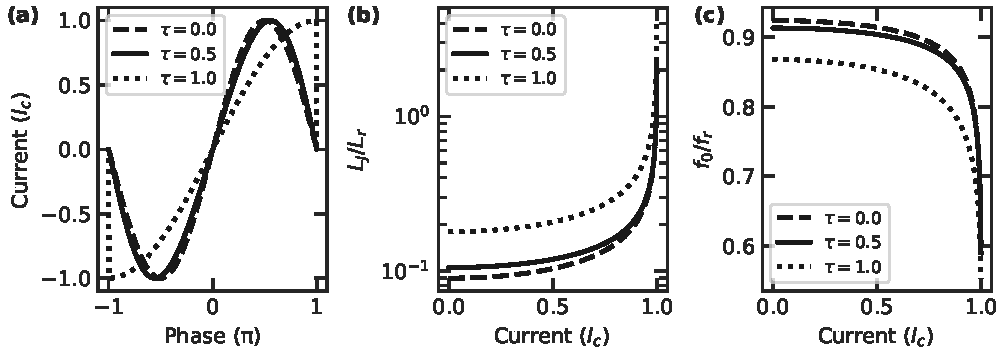
\includegraphics[width=\linewidth]{chapter-gJJ-CPR/figs/SMFigure-influence}
	\caption{
		\textbf{Predicted influence of the junction transparency on the bias current dependence.}
		%
		\textbf{(a)} CPR for various $\tau=0$ (solid), $\tau=0.5$ (dashed) and $\tau=1.0$	(dash-dotted).
		%
		\textbf{(b-c)} Josephson inductance \textbf{(b)} and resonance frequency \textbf{(c)} supercurrent for	same transparencies as in \textbf{(a)}.
		%
		Increased junction transmission leads to forward skewing of the CPR, thus a reduced slope and higher Josephson inductance, which in turn reduces the resonance frequency and increases the tuning.
	}
	\label{fig:SMinfluence}
\end{figure}

Without any knowledge on the junction transparency $\tau$, fitting data of a CPW cavity with JJ exhibiting a potentially nonsinusoidal CPR can lead to significant deviations from the true circuit parameters.
%
In Fig.~\ref{fig:SMtau}, we demonstrate the effect of $\tau$ on the extracted circuit parameters:
%
If the JJ shorting the CPW to ground has a forward skewed CPR, i.e. $\tau>0$, and Eq.~\ref{eq:Pogorzalek} is used to fit this data (dashed lines in Fig.~\ref{fig:SMtau}) under the assumption of a JJ with purely sinusoidal CPR, the extracted values (solid lines) for $f_r$ and $L_r$ will be too small compared with the true values, while $I_c$ will appear to be larger than expected, with consequently lower $L_J$.
%
Naively, one would assume the RF measurement to result in $L_J$ to be larger than the value expected from DC measurements due to the increased inverse CPR slope for identical $I_c$.
%
Nonetheless, the fit model accounting for the resonator tunability results in the opposite behavior.

To fit the bias current dependence data for extracting $\tau$, we first keep $\tau$ fixed and compare the fit residuals for various $\tau\in[0,1]$, cf. Fig.~\ref{fig:SMres}(a).
%
In a second step, we set $\tau$ as additional free parameter with the best results for $f_r$, $L_r$ and $I_c$, and set the initial value of $\tau$ as the one with previously determined minimum reduced $\chi^2$.
%
The fit converges more reliably than by setting $\tau$ as free parameter from the start, since this way the fit does not get trapped in a local minima.

Both current and frequency noise, however, can result in artificial global minima in $\chi^2(\tau)$, as shown in Fig.~\ref{fig:SMres}(b-c).
%
For a critical current of \SI{2}{\micro\ampere} and bias currents up to $0.9I_c$, already $\sigma_I\geq\SI{1}{\nano\ampere}$ is enough to significantly throw off the fit for low values of $\tau$.
%
Frequency noise of $\sigma_f<\SI{1}{\mega\hertz}$ has no influence on the fitting algorithm.
%
As the responsivity $\partial f_0/\partial I_b$ increases with $I_b$, so does the frequency noise for a fixed current noise, cf. Fig.~\ref{fig:SMres}(d).
%
From the average data fluctuations and comparing these with the expected $\sigma_f(\sigma_I)$, we estimate $\sigma_I<\SI{1}{\nano\ampere}$ in our setup.
%
We therefore conclude that our fitting algorithm should present a reliable way of extracting $\tau$. 

\begin{figure}
	\centering
	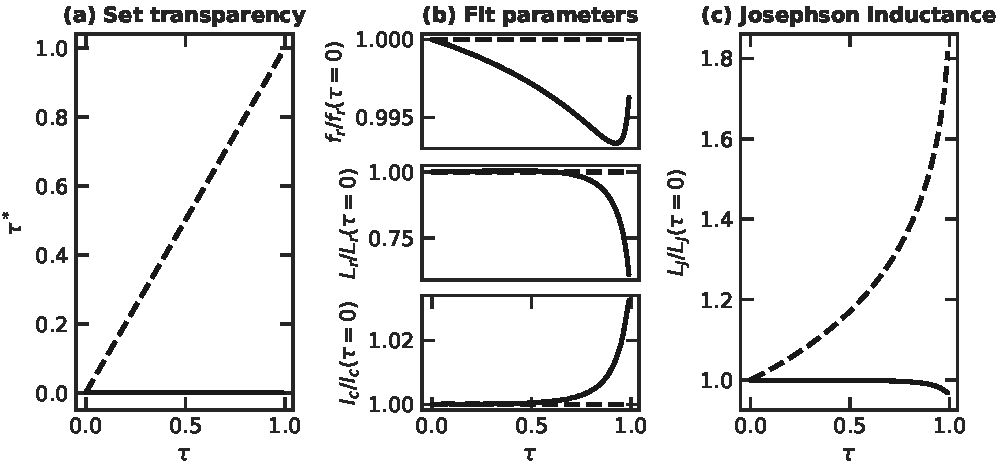
\includegraphics[width=\linewidth]{chapter-gJJ-CPR/figs/SMFigure-tauparams}
	\caption{
		\textbf{Influence of $\tau$ on extracted fit parameters with Eq.~\ref{eq:Pogorzalek}.}
		Increasing $\tau$ (dashed line in \textbf{(a)}) results in a larger $L_J$ (dashed line in \textbf{(e)}), while the other fit parameters (dashed lines in \textbf{(b-d)}) remain constant.
		%
		In order for a fit model using Eq.~\ref{eq:Pogorzalek} under the assumption of a sinusoidal CPR (solid lines) to reproduce the data (points), significant deviations from the true parameters occur.
		%
		Specifically, the fit model returns a larger critical current than expected which leads to a reduced calculated $L_J$, even though the real $L_J$ increases with $\tau$.
	}
	\label{fig:SMtau}
\end{figure}

\begin{figure}
	\centering
	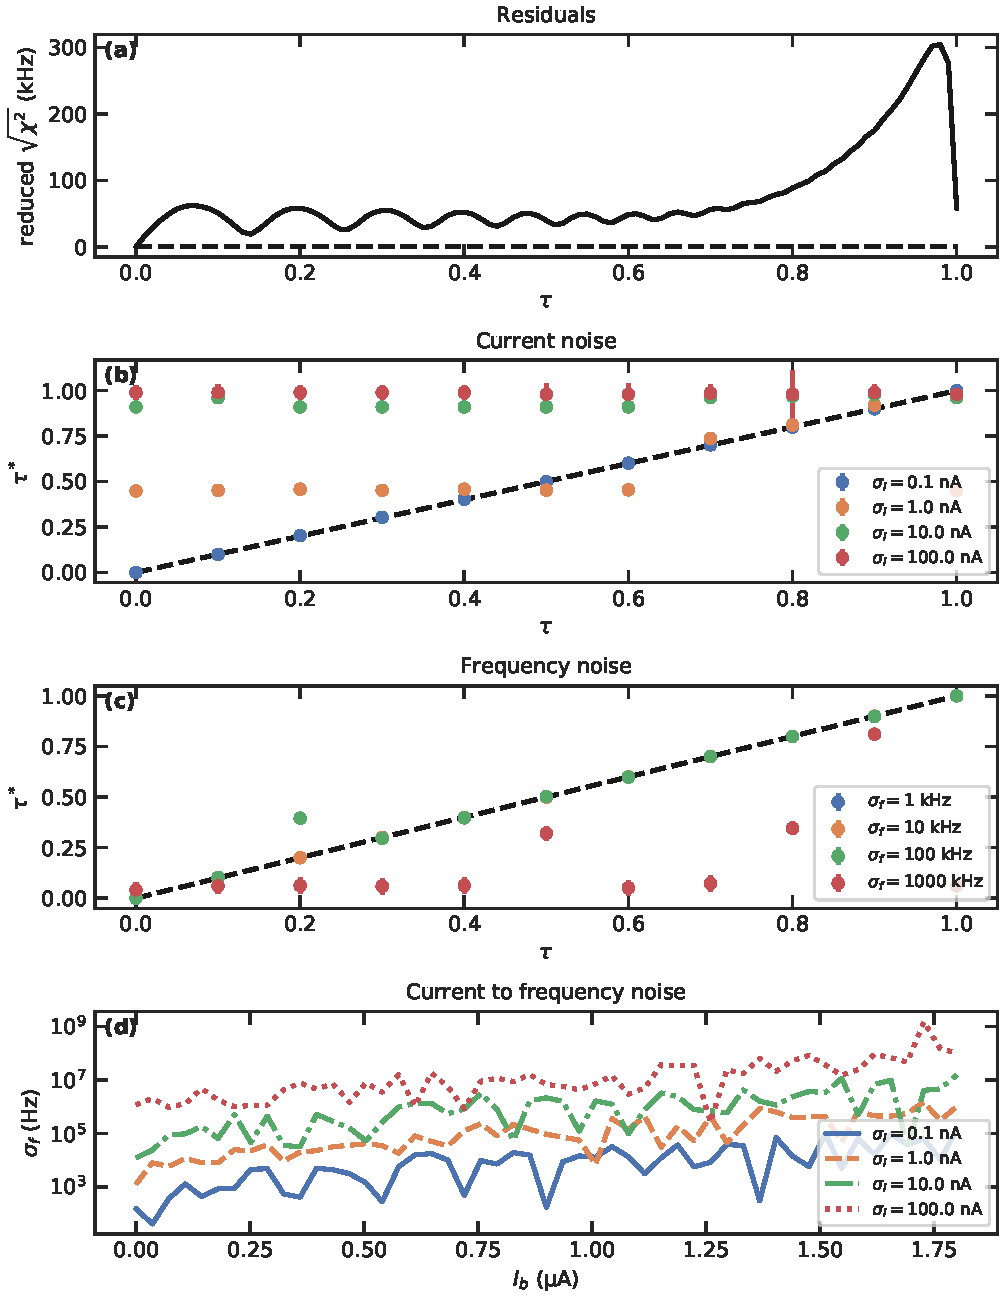
\includegraphics[width=\linewidth]{chapter-gJJ-CPR/figs/SMFigure-noise}
	\caption{
		\textbf{Influence of $\tau$ and noise on fit result.}
		\textbf{(a)} Assuming a sinusoidal CPR for Eq.~\ref{eq:Pogorzalek} to fit data originating from a forward skewed CPR results in minimum fit residuals for $\tau=0$ (solid line).
		%
		Assuming the correct $\tau$ however results in minimum residuals (dashed line).
		%
		\textbf{(b-d)} Both current and frequency noise can significantly throw off the fitting algorithm by creating artificially global residual minima.
		%
		Plotted are calculations for $I_c=\SI{2}{\micro\ampere}$.
		%
		We estimate $\sigma_I<\SI{1}{\nano\ampere}$ in our setup.
	}
	\label{fig:SMres}
\end{figure}

\references{dissertation}

